\documentclass[11pt]{article}

\usepackage[margin=1in]{geometry}
\usepackage{amsmath}
\usepackage{booktabs}
\usepackage{graphicx}
\usepackage[hidelinks]{hyperref}

\title{Power Profile of a Cyclist:\\ Pacing and Performance over Time-Trial Courses}
\author{Carter Dandridge \and (add teammates)}
\date{\today}

\begin{document}
\maketitle

% ====================================================================
% SUMMARY SHEET (one page) -- WRITE THIS LAST, AND WRITE IT YOURSELVES.
% ====================================================================
\section*{Summary}
% TODO (write yourselves, last): a standalone one-page overview that makes a
% reader want to continue. NOT a restatement of the problem. Cover what we
% modelled, the headline findings (value of pacing, the rider x course
% cross-over, wind sensitivity), and what they mean.

% ====================================================================
\section{Introduction}

\subsection{Background}
% TODO (write yourselves): concise background on individual time trials and why
% pacing, rider type, and terrain matter.

\subsection{Problem restatement}
% TODO (write yourselves, in your own words): in an individual time trial a
% rider covers a fixed course alone; given the rider's power curve, how should
% power be distributed over the course to minimise time, under a finite energy
% budget and accumulating fatigue?

\subsection{Variables and notation}
\begin{center}
\begin{tabular}{cl}
\toprule
Symbol & Meaning \\
\midrule
$P_i$ & rider power on segment $i$ (W) \\
$v_i$ & steady speed on segment $i$ (m/s) \\
$d_i$ & segment length (m) \\
$\mathrm{grade}_i$ & segment slope (fraction) \\
$w_i$ & segment headwind (m/s) \\
$\tau_i$ & turn penalty on segment $i$ (s) \\
$\rho$ & air density (kg/m$^3$) \\
$C_dA$ & drag area (m$^2$) \\
$C_{rr}$ & rolling-resistance coefficient \\
$m$ & rider $+$ bike mass (kg) \\
$g$ & gravitational acceleration (m/s$^2$) \\
$\mathrm{CP}$ & critical power (W) \\
$W'$ & anaerobic work capacity (J) \\
\bottomrule
\end{tabular}
\end{center}

\subsection{Assumptions}
% These are the assumptions the model actually makes. TODO (write yourselves):
% JUSTIFY each one -- the rubric grades the justification, not just the list.
\begin{enumerate}
  \item Steady speed within each segment (no within-segment acceleration).
  \item Small-angle slope: $\sin\theta \approx \mathrm{grade}$ and $\cos\theta \approx 1$.
  \item Each rider is a critical-power model (a sustainable $\mathrm{CP}$ plus a finite reserve $W'$).
  \item $W'$ drains at rate $P-\mathrm{CP}$ above CP and refills below it, linearly and symmetrically, and never goes negative.
  \item Wind enters as an effective scalar headwind per segment.
  \item Turns cost a fixed time penalty (no explicit deceleration/acceleration).
\end{enumerate}

\subsection{Modelling approach}
% TODO (write yourselves): one paragraph on why a segment-wise power balance
% plus a CP/W' pacing layer is a reasonable approach to this problem.

% ====================================================================
\section{The model}

For each segment $i$, the rider's power must overcome aerodynamic drag, rolling
resistance, and gravity to hold a steady speed $v_i$:
\begin{equation}
P_i = v_i\!\left[\tfrac{1}{2}\,\rho\,C_dA\,(v_i + w_i)^2 + C_{rr}\,m\,g + m\,g\,\mathrm{grade}_i\right].
\label{eq:power}
\end{equation}
Given the rider's power, Eq.~\eqref{eq:power} is solved for $v_i$ numerically
(it is cubic in $v_i$). The segment time and total race time are
\begin{equation}
T_i = \frac{d_i}{v_i} + \tau_i, \qquad
T_{\mathrm{total}} = \sum_i T_i .
\label{eq:time}
\end{equation}

\subsection{Rider model and pacing}
Each rider holds critical power $\mathrm{CP}$ for a long time and carries a
finite anaerobic reserve $W'$. Riding at power $P$ for time $t$ changes the
reserve by $-(P-\mathrm{CP})\,t$: it drains above CP, refills below, and may
never go negative --- this is the rider's energy/fatigue limit. We compare
holding CP the whole way (reserve unspent) against spending $W'$ on the slowest
segments (climbs and headwinds).
% TODO (write yourselves): explain WHY spending the reserve where the rider is
% slowest saves the most time, and how the assumptions above enter the model.

% ====================================================================
\section{Results}
% TODO (write yourselves): interpret each table and figure -- what the numbers
% MEAN, not just what they are. The figures are generated by src/plots.py into
% paper/figures/; you still need to explain each one in the text.

\begin{table}[h]\centering
\caption{Pacing vs.\ constant power (custom course, male TT specialist).}
\begin{tabular}{lr}
\toprule
Strategy & Time (s) \\
\midrule
Constant CP & 440.9 \\
Paced (spend $W'$ on slow sections) & 405.8 \\
\midrule
Saved & 35.1 \\
\bottomrule
\end{tabular}
\end{table}

\begin{figure}[h]\centering
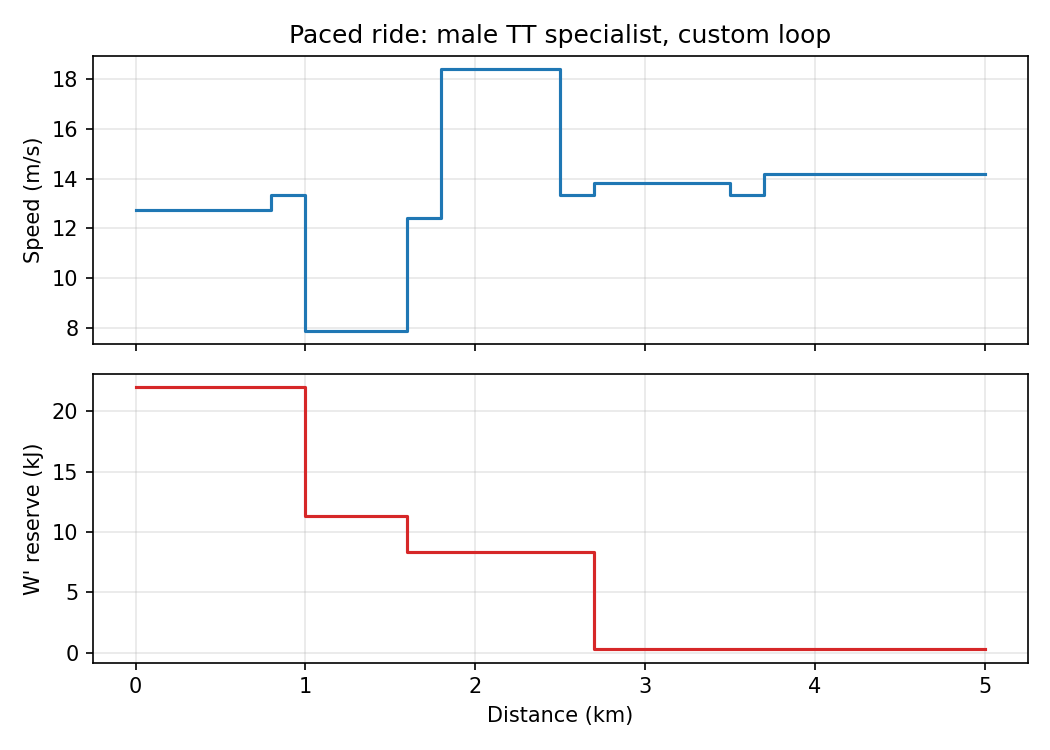
\includegraphics[width=0.8\textwidth]{figures/pacing_profile.png}
\caption{Speed and remaining $W'$ reserve along the custom loop for the paced ride.}
\end{figure}

\begin{table}[h]\centering
\caption{Rider $\times$ course: climber minus TT-specialist finishing time (s); negative means the climber is faster.}
\begin{tabular}{lrrr}
\toprule
 & Custom & Tokyo (hilly) & Flanders (flat) \\
\midrule
Male   & $+8.5$  & $-21.6$ & $+56.8$  \\
Female & $+14.9$ & $+6.8$  & $+174.0$ \\
\bottomrule
\end{tabular}
\end{table}

\begin{figure}[h]\centering
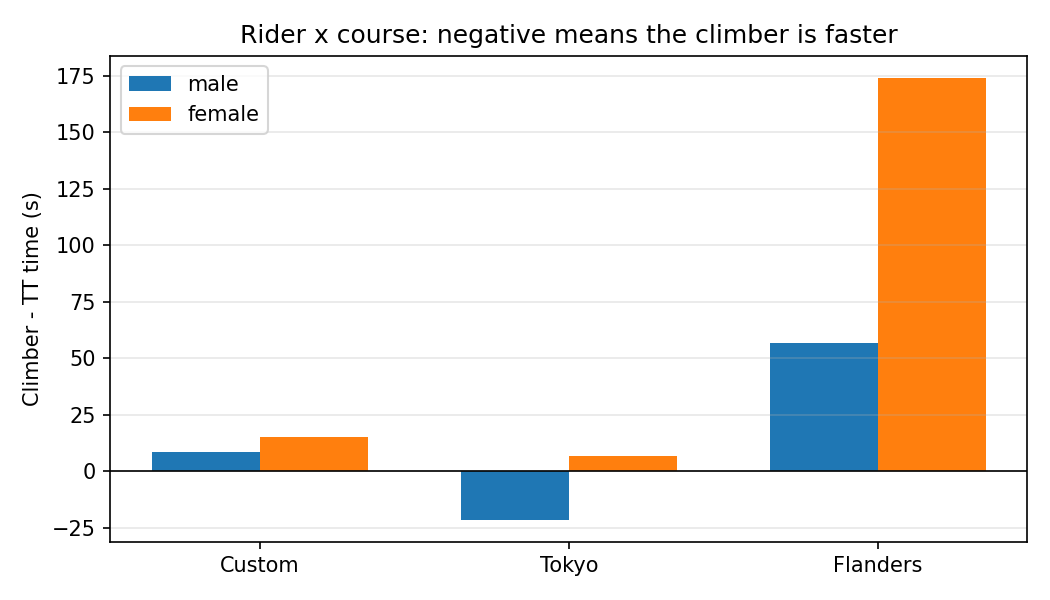
\includegraphics[width=0.8\textwidth]{figures/crossover.png}
\caption{Climber minus TT-specialist finishing time, by course (negative = climber faster).}
\end{figure}

\begin{table}[h]\centering
\caption{Wind sensitivity: one fixed plan held into different winds (custom course, male TT specialist). ``Reserve blown'' = the planned effort is no longer feasible.}
\begin{tabular}{lrl}
\toprule
Wind & Time (s) & vs.\ still \\
\midrule
4 m/s tailwind & 347.5 & $-58.3$ \\
2 m/s tailwind & 374.5 & $-31.3$ \\
still          & 405.8 & $0.0$ \\
2 m/s headwind & 441.9 & $+36.1$ (reserve blown) \\
4 m/s headwind & 483.5 & $+77.7$ (reserve blown) \\
\bottomrule
\end{tabular}
\end{table}

\begin{figure}[h]\centering
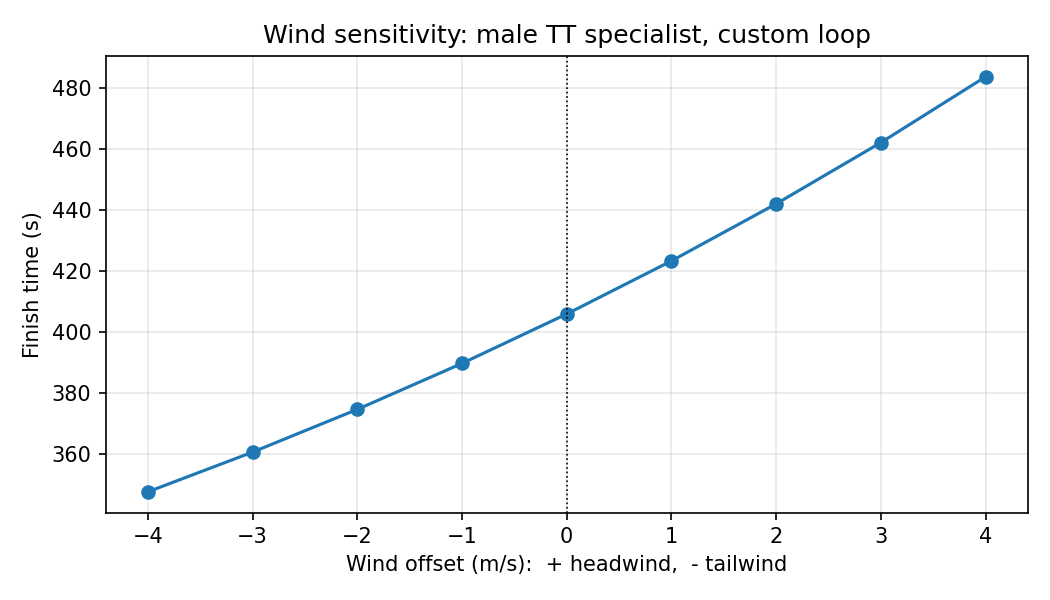
\includegraphics[width=0.7\textwidth]{figures/wind_sensitivity.png}
\caption{Finish time vs.\ a uniform wind offset (custom course, male TT specialist).}
\end{figure}

\begin{table}[h]\centering
\caption{Sensitivity to missing the target power: rider holds $(1{+}\mathrm{dev})$ of the planned power on every segment (custom course, male TT specialist).}
\begin{tabular}{lrl}
\toprule
Deviation & Time (s) & vs.\ plan \\
\midrule
$-10\%$ & 423.7 & $+17.9$ \\
$-5\%$  & 414.4 & $+8.6$ \\
$0\%$   & 405.8 & $0.0$ \\
$+5\%$  & 397.9 & $-7.9$ (reserve blown) \\
$+10\%$ & 390.5 & $-15.2$ (reserve blown) \\
\bottomrule
\end{tabular}
\end{table}

\begin{table}[h]\centering
\caption{Validation: model (male TT archetype, CP 350 W) vs.\ the actual men's winners.}
\begin{tabular}{lrrr}
\toprule
Course & Model (s) & Winner (s) & Gap \\
\midrule
Tokyo (2 laps, 44.2 km) & 4203 & 3304 (Rogli\v{c}) & $+27\%$ \\
Flanders (43.3 km)      & 3425 & 2868 (Ganna)      & $+19\%$ \\
\bottomrule
\end{tabular}
\end{table}

\begin{figure}[h]\centering
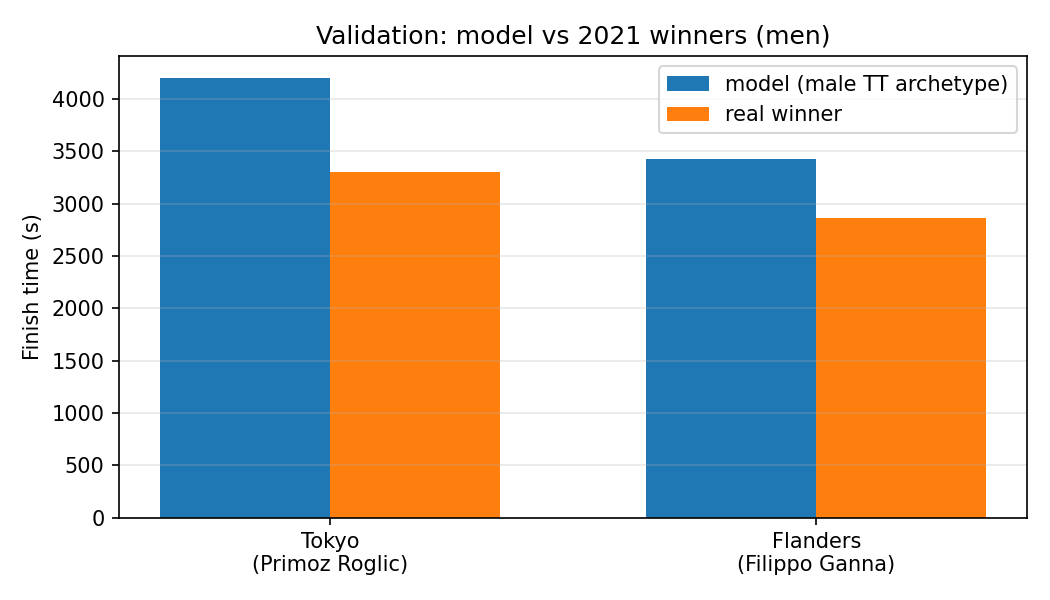
\includegraphics[width=0.7\textwidth]{figures/validation.png}
\caption{Model finishing time vs.\ the 2021 men's winners, by course.}
\end{figure}

% ====================================================================
\section{Model assessment}
% TODO (write yourselves): strengths and weaknesses against the problem goals;
% where the model is likely to fail; how it could be tested, calibrated, or
% improved with more data.

\paragraph{Known limitations and possible refinements.}
\begin{itemize}
  \item The pacing heuristic spends the reserve uniformly across below-average-speed segments; truly time-optimal pacing would weight power toward the slowest segment.
  \item No blow-up dynamics: when $W'$ empties, the plan is flagged infeasible rather than the rider slowing.
  \item Wind is treated as a scalar headwind, not a direction-dependent vector.
  \item $W'$ recovery is modelled as linear and symmetric with depletion.
\end{itemize}
% TODO (write yourselves): pick at least one refinement (e.g. optimal pacing
% allocation) and discuss how it would change the results -- the rubric
% explicitly requires considering one alternative modelling choice.

% ====================================================================
\section{Conclusion}
% TODO (write yourselves): summarise the findings and give future directions.

% ====================================================================
\section*{References}
% TODO: format these properly (the citation style is your choice). Full list
% with URLs is in references/data-sources.md:
%  - 2021 Tokyo Olympic and Flanders Worlds ITT results and routes
%    (Wikipedia, Cyclingnews, cyclingstage.com)
%  - Critical power / W' ranges (PMC8562202)
%  - CdA and Crr ranges (BestBikeSplit)

\end{document}
